Al planificar una arquitectura escalable, necesitamos tener una forma de agregar o quitar nodos de manera dinámica de forma que se logre elasticidad para ecalar horizontalmente. La forma más común de lograr esto es utilizando un nodo dedicado a la distribución del trabajo entrante entre aquellos capaces de atender la tarea entrante, lo cual no solo abstrae a las capas anteriores de la arquitectura sobre cuántos o qué nodos se encargan de realizar ese trabajo, si no que además permite distribuir más equitativamente esa carga entre ellos.

Esta forma de balanceo y escalabilidad horizontal es la que utilizaremos en nuestra propuesta, y a tal fin hemos considerado como opciones las dos herramientas de código abierto más populares y probadas de los últimos años. En los apartados presentados a continuación analizaremos brevemente cada una a fin de elegir una para utilizar en nuestra propuesta. En la figura \autoref{fig:netcraft-stats-web-servers} se puede que del millón de sitios web más concurridos, los dos primeros servidores web que se utilizan son \nameref{soa:tecnologias:apache} y \nameref{soa:tecnologias:nginx}, con una tendencia en alza de este último, según datos del sitio \textit{netcraft}\footnote{\url{http://news.netcraft.com/archives/2016/01/26/january-2016-web-server-survey.html}}.

\begin{figure}[H]
  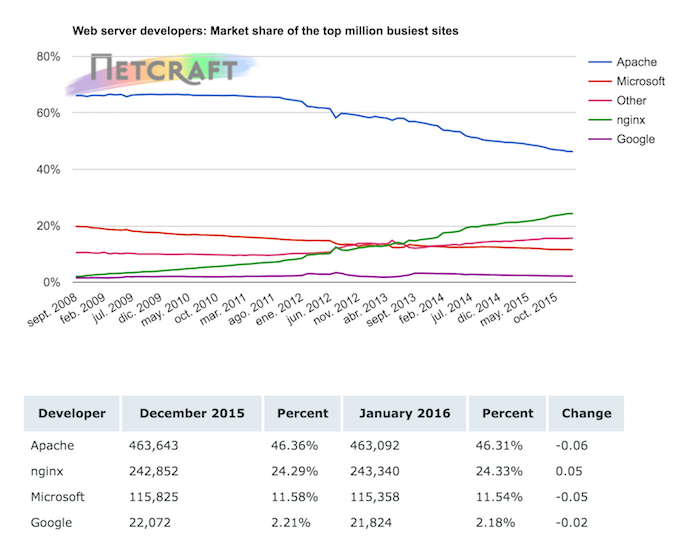
\includegraphics[width=\linewidth]{src/images/03-capitulo-3/tecnologias/balanceo/stats.png}
  \caption{Resultados de la encuesta de uso de servidores web de netcraft, Enero 2016}
  \label{fig:netcraft-stats-web-servers}
\end{figure}
